% RQ3 Results: Proposal Pipeline Effects

\subsection{Overview}

We present results from \experimentruns{} simulation runs across 9 pipeline configurations.

\begin{table}[htbp]
\centering
\caption{RQ3 Results Overview (Experiment 05)}
\label{tab:rq3-overview}
\begin{tabular}{lr}
\toprule
Parameter & Value \\
\midrule
Pipeline configurations & 9 \\
Runs per configuration & 30 \\
Total simulation runs & 270 \\
\bottomrule
\end{tabular}
\end{table}

\subsection{Temp-Check Effects}

\subsubsection{Filtering Effectiveness}

\begin{figure}[htbp]
    \centering
    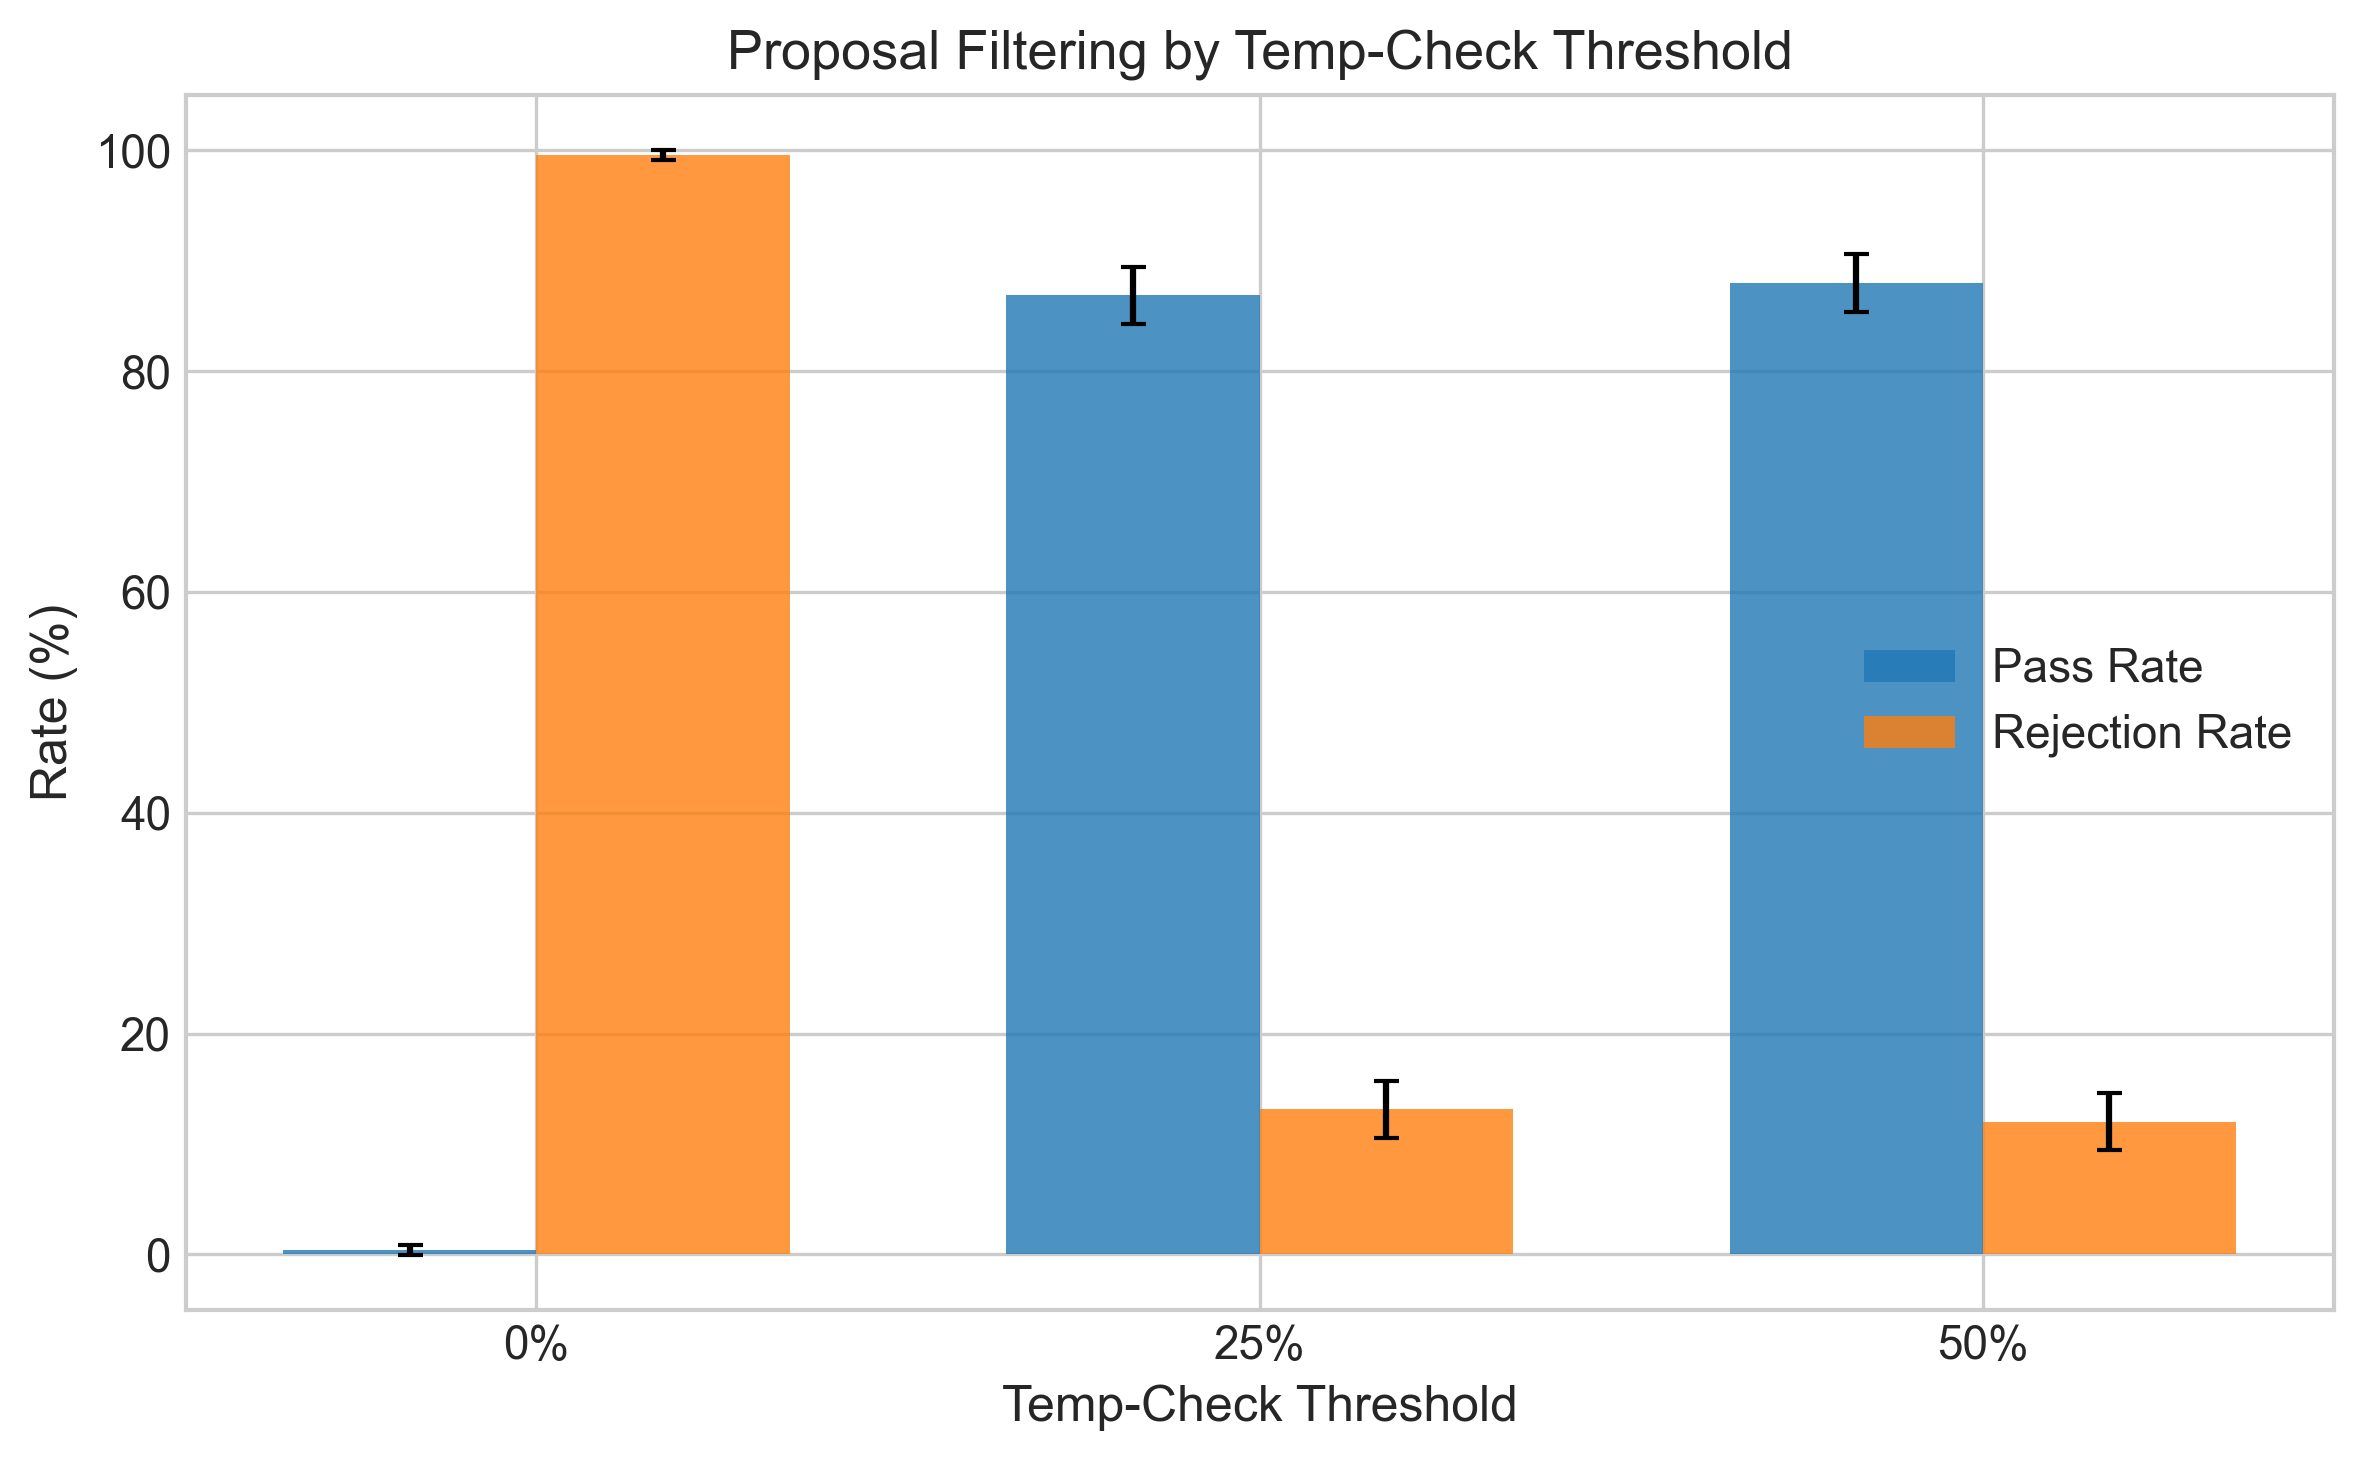
\includegraphics[width=0.8\textwidth]{../figures/rq3_tempcheck}
    \caption{Effect of temp-check threshold on proposals reaching formal voting. Higher thresholds reduce formal voting load but also filter some viable proposals.}
    \label{fig:rq3-tempcheck}
\end{figure}

\begin{table}[htbp]
\centering
\caption{Temp-check filtering outcomes}
\label{tab:rq3-tempcheck}
\begin{tabular}{lcccc}
\toprule
Threshold & Conversion & Formal Pass Rate & Abandonment & False Negative \\
\midrule
\pl{None} & \pl{--} & \pl{--} & \pl{--} & \pl{--} \\
\pl{20\%} & \pl{--} & \pl{--} & \pl{--} & \pl{--} \\
\pl{40\%} & \pl{--} & \pl{--} & \pl{--} & \pl{--} \\
\bottomrule
\end{tabular}
\end{table}

\subsubsection{Quality Improvement}

\begin{figure}[htbp]
    \centering
    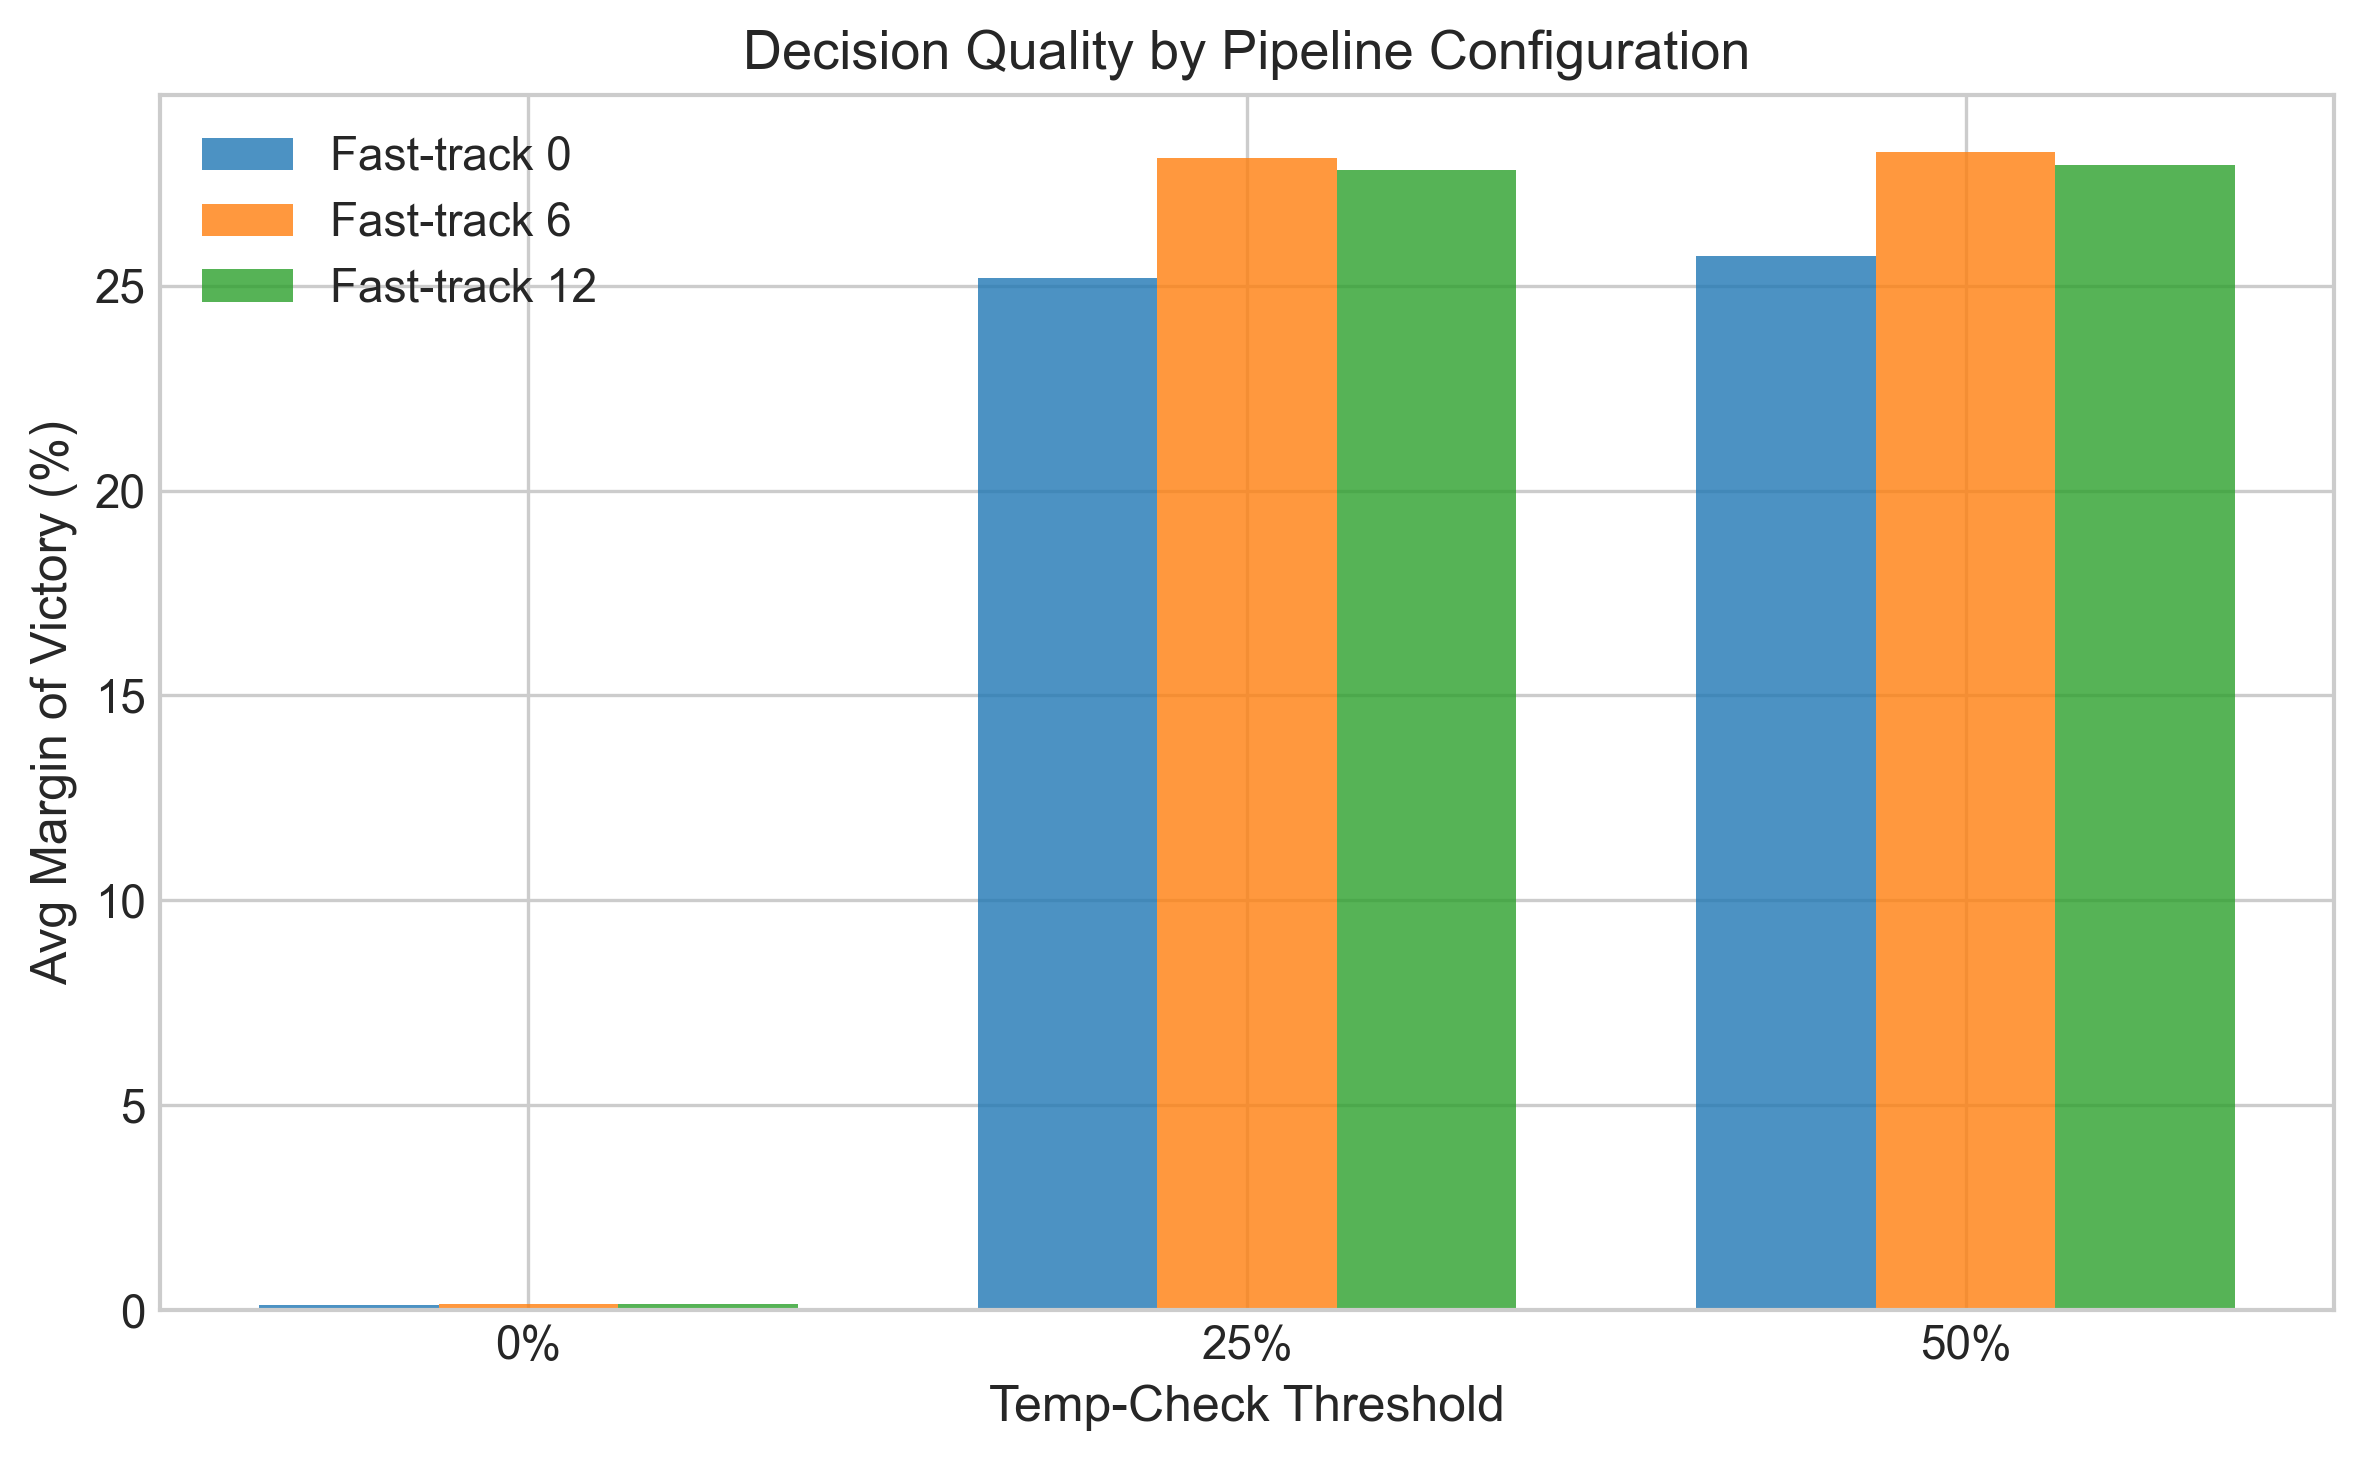
\includegraphics[width=0.8\textwidth]{../figures/rq3_quality}
    \caption{Pass rate of proposals reaching formal voting vs. temp-check threshold. Higher thresholds correlate with higher-quality (more likely to pass) proposals reaching formal stage.}
    \label{fig:rq3-quality}
\end{figure}

\subsection{Fast-Track Effects}

\subsubsection{Time-to-Decision Distribution}

\begin{figure}[htbp]
    \centering
    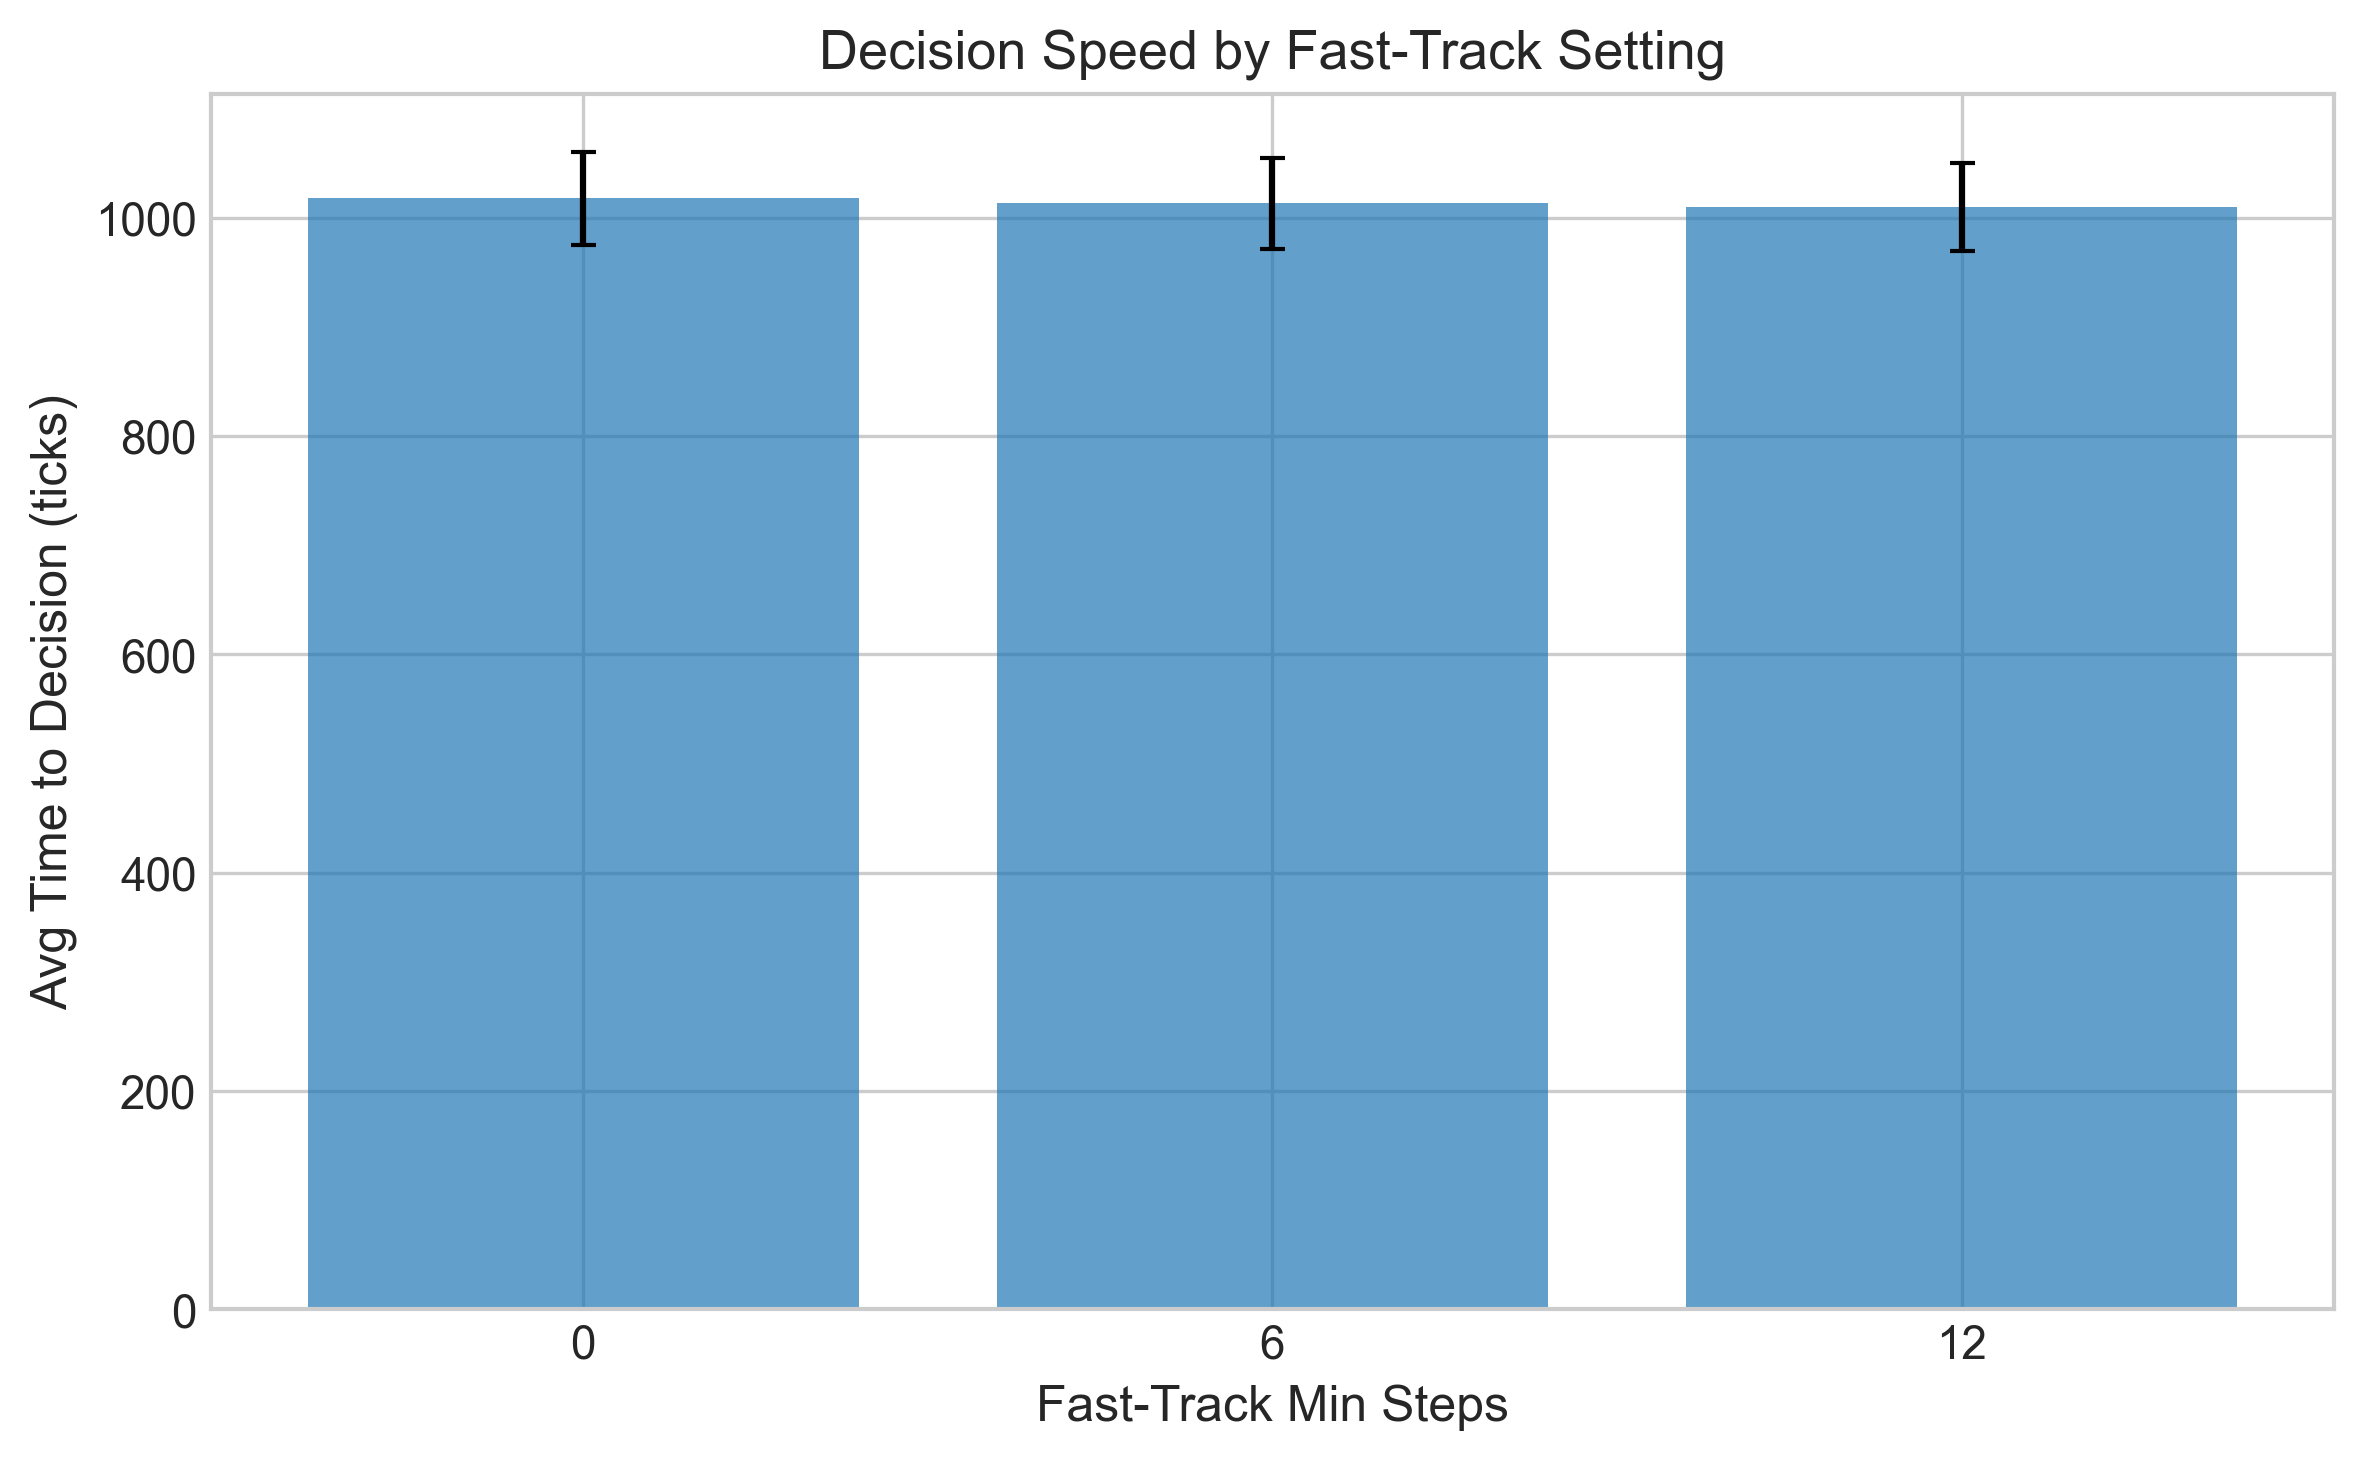
\includegraphics[width=0.8\textwidth]{../figures/rq3_ttd}
    \caption{Time-to-decision distribution under different fast-track settings. Fast-tracks create bimodal distribution: quick resolution for qualifying proposals, standard timeline for others.}
    \label{fig:rq3-ttd}
\end{figure}

\begin{table}[htbp]
\centering
\caption{Fast-track effects on time-to-decision}
\label{tab:rq3-fasttrack}
\begin{tabular}{lccc}
\toprule
Setting & Mean TTD & Median TTD & Fast-Track Rate \\
\midrule
\pl{None} & \pl{--} & \pl{--} & \pl{0\%} \\
\pl{70\%} & \pl{--} & \pl{--} & \pl{--} \\
\pl{85\%} & \pl{--} & \pl{--} & \pl{--} \\
\bottomrule
\end{tabular}
\end{table}

\subsection{Expiry Effects}

\subsubsection{Abandonment and Expiry Rates}

\begin{figure}[htbp]
    \centering
    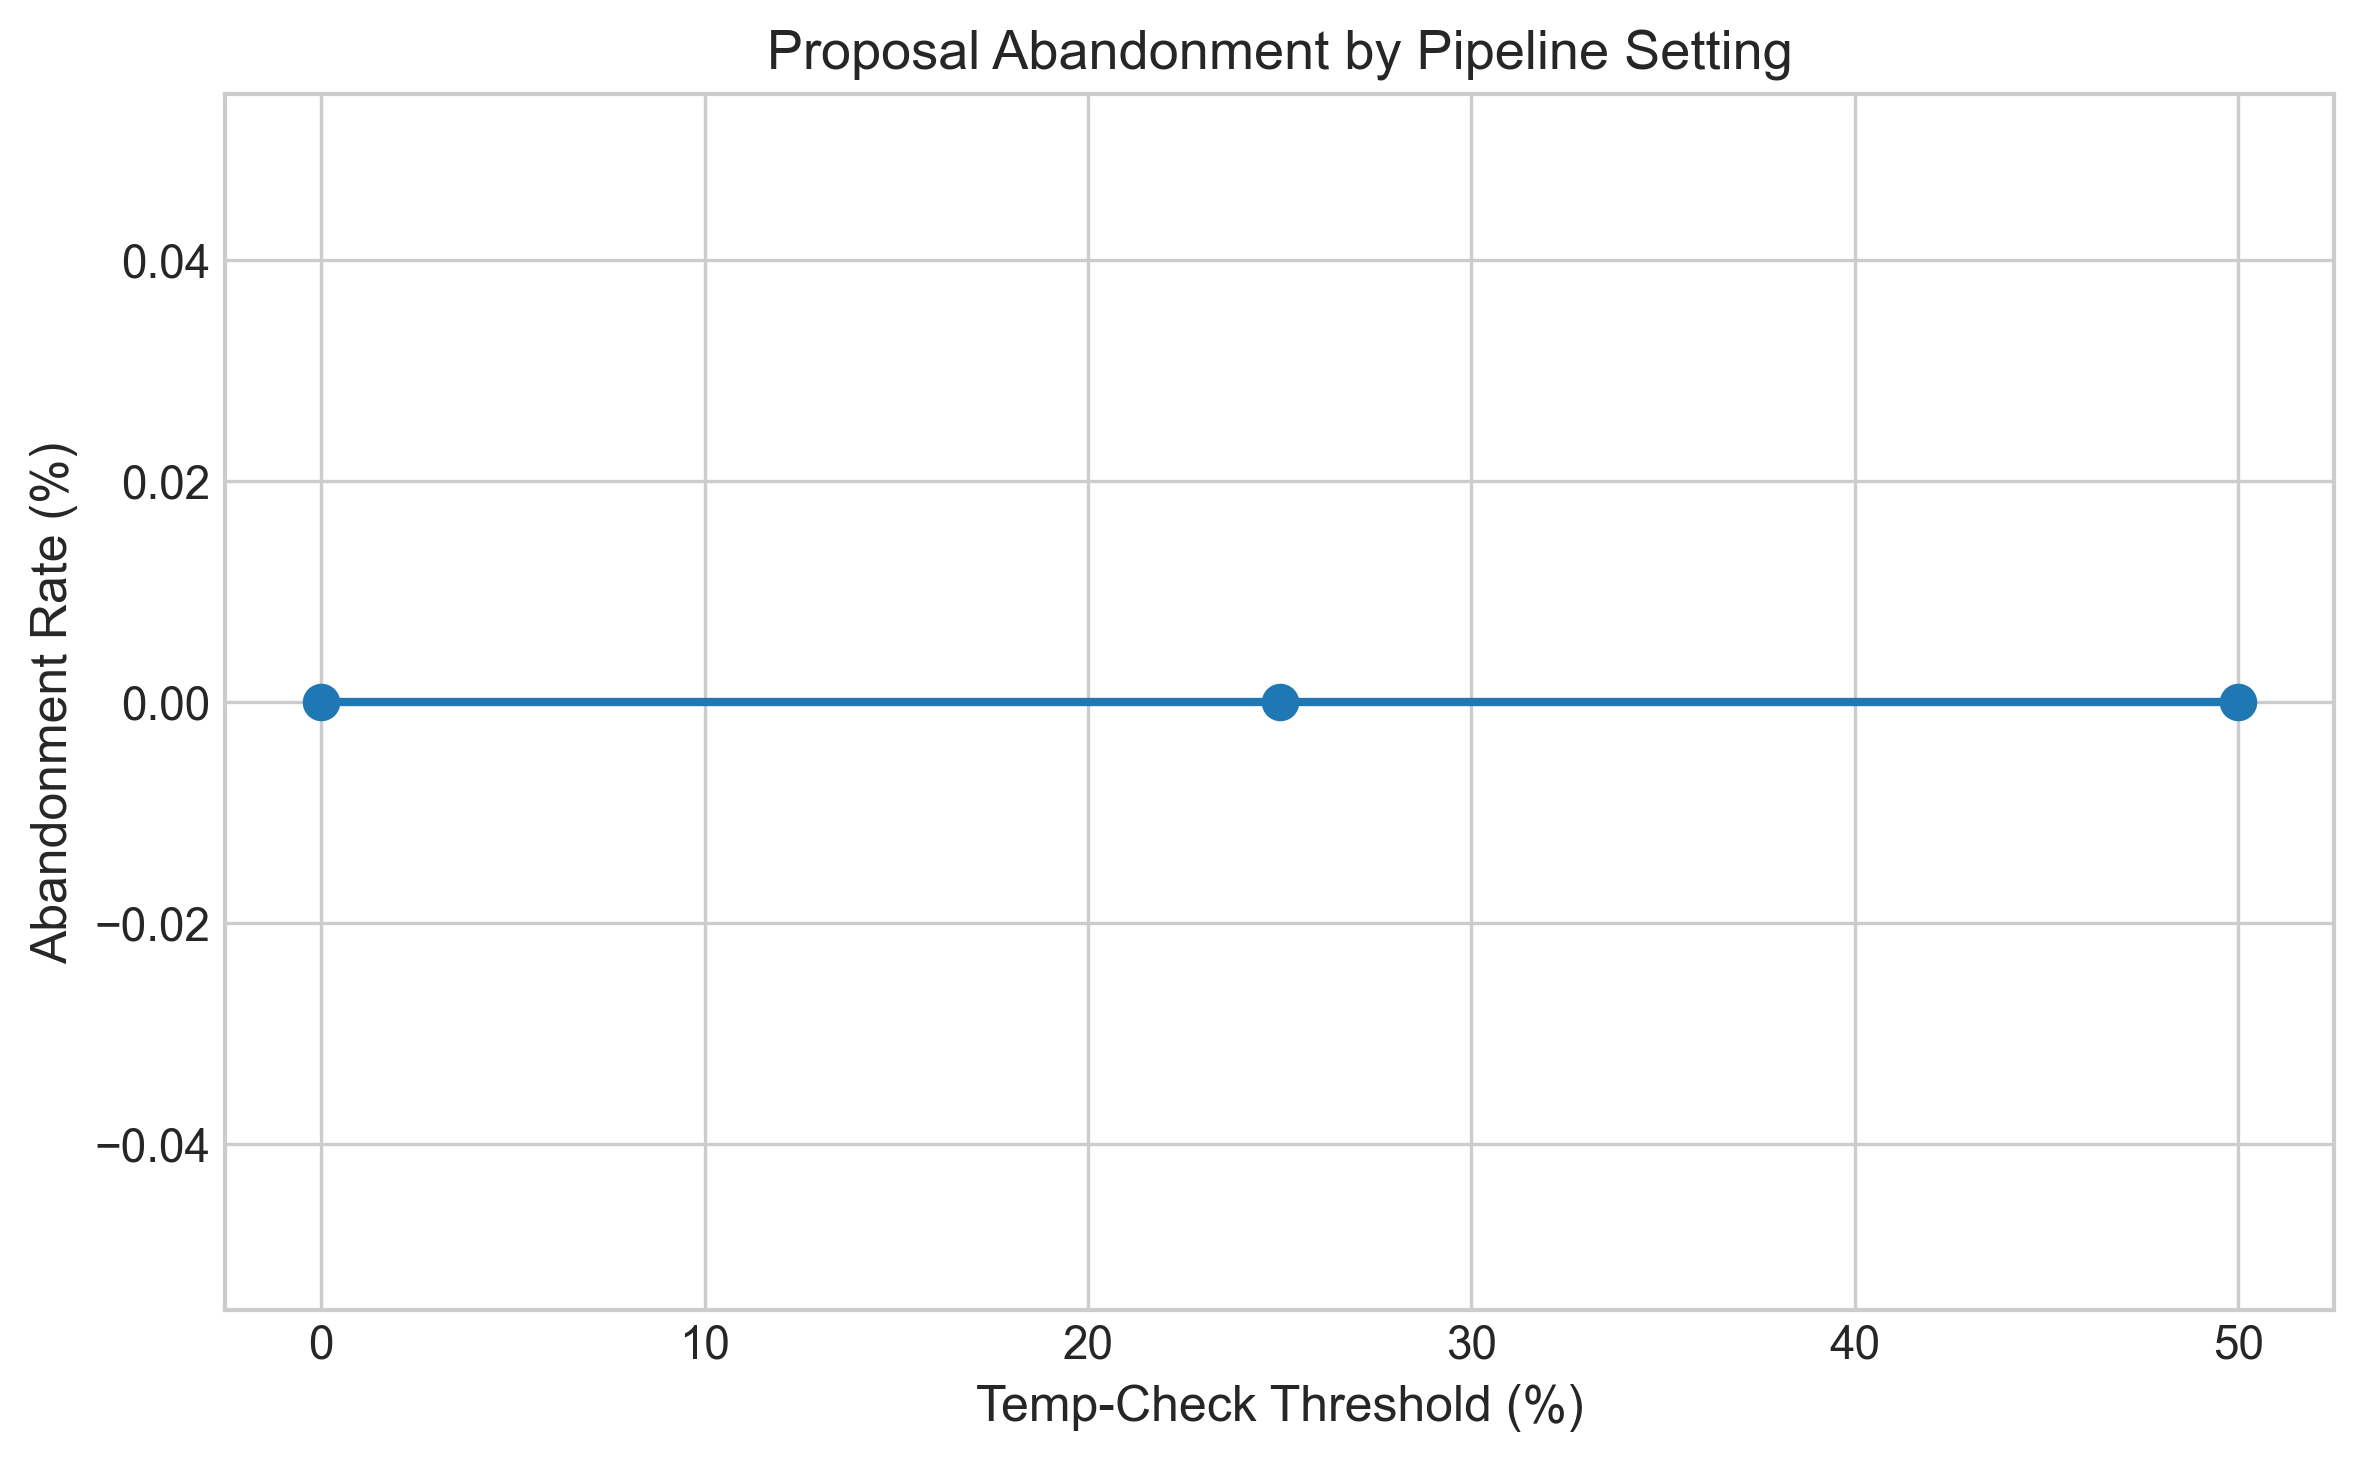
\includegraphics[width=0.8\textwidth]{../figures/rq3_expiry}
    \caption{Abandonment and expiry rates by expiry window setting. Tighter windows increase both abandonment (proposers give up) and forced expiry.}
    \label{fig:rq3-expiry}
\end{figure}

\begin{table}[htbp]
\centering
\caption{Expiry window effects}
\label{tab:rq3-expiry}
\begin{tabular}{lccc}
\toprule
Window & Abandonment Rate & Expiry Rate & Resolution Rate \\
\midrule
\pl{30 days} & \pl{--} & \pl{--} & \pl{--} \\
\pl{60 days} & \pl{--} & \pl{--} & \pl{--} \\
\pl{90 days} & \pl{--} & \pl{--} & \pl{--} \\
\bottomrule
\end{tabular}
\end{table}

\subsection{Interaction Effects}

\begin{figure}[htbp]
    \centering
    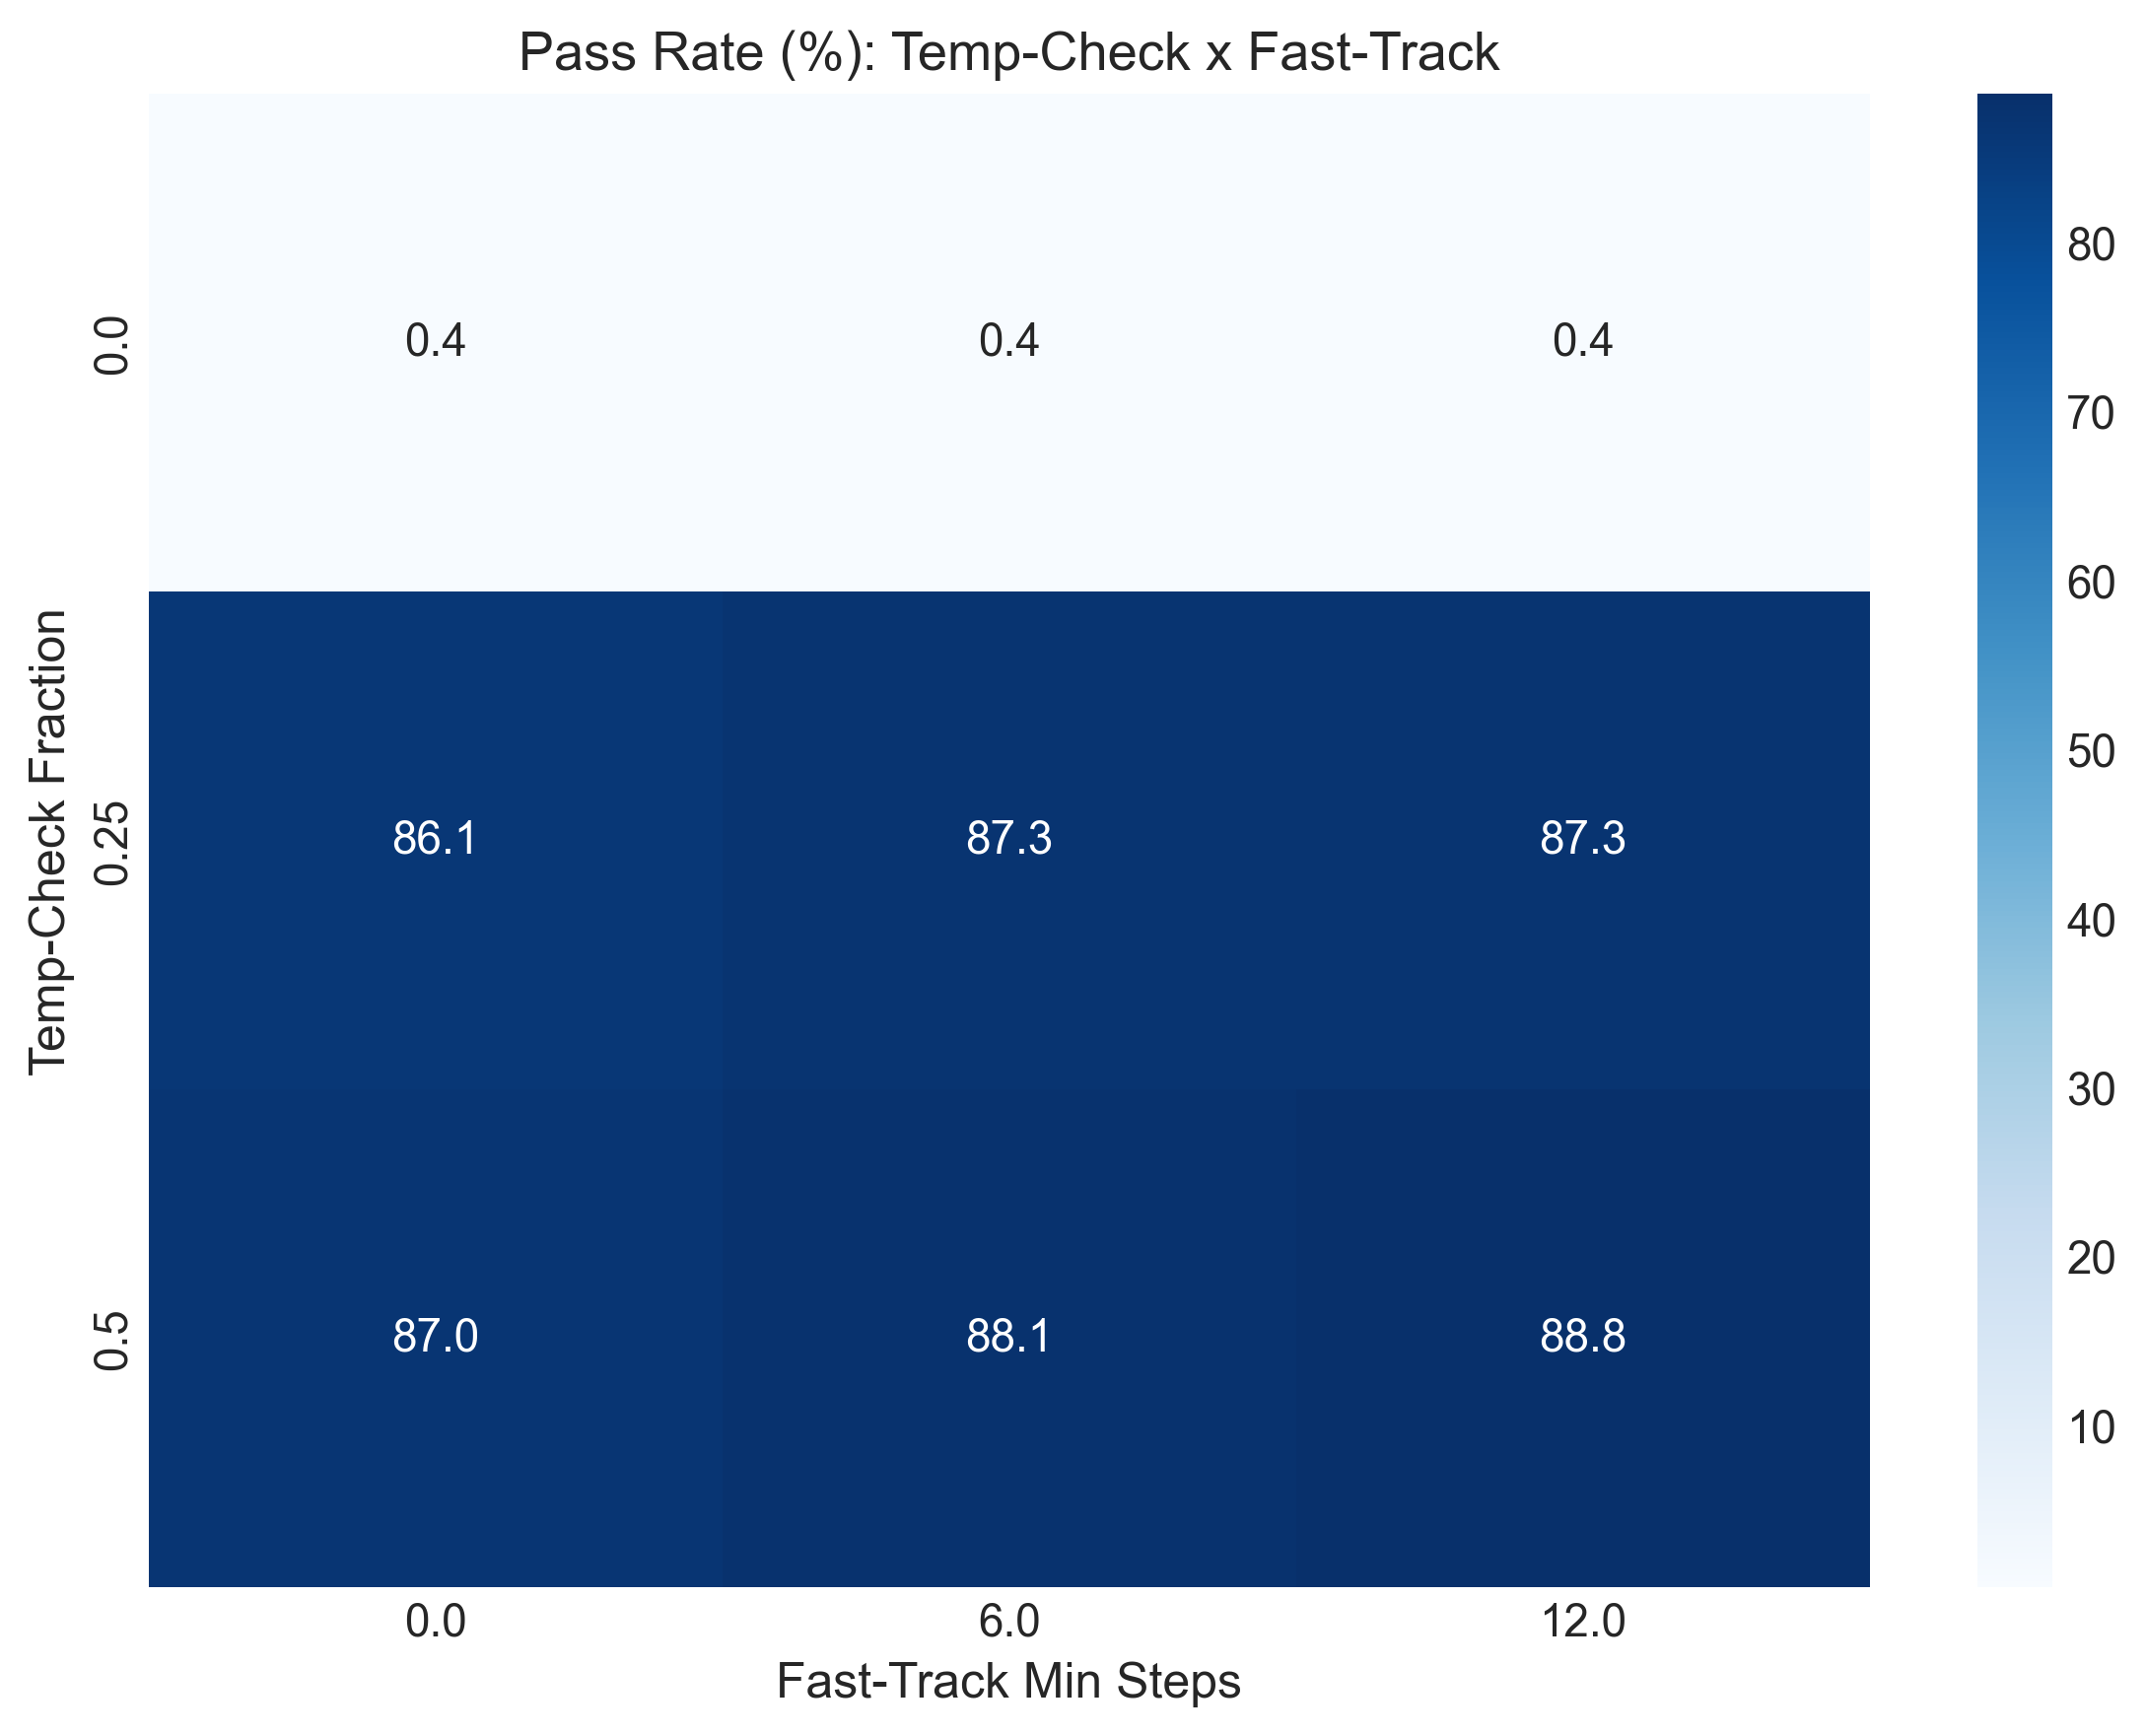
\includegraphics[width=0.8\textwidth]{../figures/rq3_interactions}
    \caption{Interaction between temp-check and fast-track settings. Moderate temp-check combined with moderate fast-track achieves best throughput-quality balance.}
    \label{fig:rq3-interactions}
\end{figure}

\subsection{Pareto Frontier}

\begin{table}[htbp]
\centering
\caption{Pareto-optimal configurations}
\label{tab:rq3-pareto}
\begin{tabular}{lllcccc}
\toprule
Config & Temp & Fast & Throughput & Pass Rate & TTD & Abandonment \\
\midrule
\pl{A} & \pl{--} & \pl{--} & \pl{--} & \pl{--} & \pl{--} & \pl{--} \\
\pl{B} & \pl{--} & \pl{--} & \pl{--} & \pl{--} & \pl{--} & \pl{--} \\
\pl{C} & \pl{--} & \pl{--} & \pl{--} & \pl{--} & \pl{--} & \pl{--} \\
\bottomrule
\end{tabular}
\end{table}

\subsection{Hypothesis Evaluation}

\begin{table}[htbp]
\centering
\caption{Hypothesis testing results}
\label{tab:rq3-hypotheses}
\begin{tabular}{llcc}
\toprule
Hypothesis & Test & $p$-value & Result \\
\midrule
H3.1: Temp-check reduces load, increases FN & Regression & \pl{--} & \pl{TBD} \\
H3.2: Fast-track reduces mean TTD & t-test & \pl{--} & \pl{TBD} \\
H3.3: Tight expiry increases abandonment & ANOVA & \pl{--} & \pl{TBD} \\
H3.4: Optimal temp-check exists & Quadratic fit & \pl{--} & \pl{TBD} \\
\bottomrule
\end{tabular}
\end{table}

\subsection{Key Findings}

\begin{enumerate}
    \item \textbf{Temp-checks improve quality at throughput cost}: Higher thresholds filter more, but proposals that pass temp-check have higher formal vote success rates

    \item \textbf{Fast-tracks effective for consensus proposals}: 70\% threshold captures most obvious winners; 85\% is too restrictive

    \item \textbf{Expiry windows matter for complex proposals}: 30-day window causes excessive abandonment; 60-90 days allows adequate deliberation

    \item \textbf{Moderate settings dominate}: Extreme configurations (no filtering OR aggressive filtering) underperform moderate approaches
\end{enumerate}
